\documentclass[12pt,a4paper]{article}
\usepackage[a4paper, margin=0.8in, headheight=14pt]{geometry}
\usepackage{fontspec}
\usepackage{unicode-math}
\setmainfont{TeX Gyre Pagella}
\setmonofont[Scale=0.88]{TeX Gyre Cursor}
\setmathfont{Latin Modern Math}
\usepackage{xcolor}
\usepackage{colortbl}
\usepackage{titlesec}
\usepackage{enumitem}
\usepackage{tabularx}
\usepackage{booktabs}
\usepackage{array}
\usepackage{amsmath}
\usepackage{tikz}
\usetikzlibrary{shapes.geometric, arrows.meta, positioning, calc, fit, decorations.pathreplacing, decorations.pathmorphing}
\usepackage{tcolorbox}
\tcbuselibrary{skins, breakable}
\usepackage{hyperref}
\usepackage{fancyhdr}
\usepackage{graphicx}
\usepackage{microtype}
\hyphenpenalty=10000
\exhyphenpenalty=10000
\sloppy
\usepackage{caption}
\usepackage{setspace}
\usepackage{multirow}
\usepackage{tocloft}
\newcommand{\Q}[1]{\textbf{#1}\par\noindent\ignorespaces}
\definecolor{myred}{RGB}{196,30,58}
\definecolor{mydark}{RGB}{30,30,50}
\definecolor{mygreen}{RGB}{14,120,80}
\definecolor{myteal}{RGB}{0,130,140}
\definecolor{myamber}{RGB}{180,100,0}
\definecolor{mypurple}{RGB}{100,30,160}
\definecolor{mygray}{RGB}{246,247,249}
\definecolor{mgframe}{RGB}{180,185,200}
\definecolor{watermark}{RGB}{145,150,170}
\definecolor{hdrred}{RGB}{250,232,235}
\definecolor{hdrgreen}{RGB}{220,244,233}
\definecolor{hdrteal}{RGB}{220,242,244}
\definecolor{hdramber}{RGB}{253,242,215}
\definecolor{hdrpurple}{RGB}{238,228,255}
\definecolor{hdrgray}{RGB}{238,240,245}
\definecolor{rowalt}{RGB}{250,251,253}

\titleformat{\section}{\large\bfseries\color{myred}}{\thesection.}{0.5em}{}[\vspace{1pt}{\color{myred}\rule{\linewidth}{0.8pt}}]
\titleformat{\subsection}{\normalsize\bfseries\color{myteal}}{\thesubsection}{0.5em}{}
\titlespacing*{\section}{0pt}{18pt}{7pt}
\titlespacing*{\subsection}{0pt}{11pt}{4pt}
\setlength{\parindent}{0pt}
\setlength{\parskip}{4pt}
\renewcommand{\cfttoctitlefont}{\large\bfseries\color{myred}}
\renewcommand{\cftaftertoctitle}{\par\noindent{\color{myred}\rule{\linewidth}{0.8pt}}}
\setlength{\cftbeforetoctitleskip}{0pt}
\setlength{\cftaftertoctitleskip}{6pt}
\renewcommand{\cftsecfont}{\normalsize\bfseries\color{mydark}}
\renewcommand{\cftsecpagefont}{\normalsize\bfseries\color{mydark}}
\renewcommand{\cftsecleader}{\cftdotfill{\cftdotsep}}
\setlength{\cftbeforesecskip}{7pt}
\renewcommand{\cftsubsecfont}{\small\color{mydark}}
\renewcommand{\cftsubsecpagefont}{\small\color{mydark}}
\setlength{\cftbeforesubsecskip}{3pt}
\setlength{\cftsubsecindent}{1.4em}
\renewcommand{\cftpartfont}{\normalsize\bfseries\color{myteal}}
\renewcommand{\cftpartpagefont}{\normalsize\bfseries\color{myteal}}
\setlength{\cftbeforepartskip}{14pt}
\renewcommand{\arraystretch}{1.45}
\setlength{\tabcolsep}{6pt}
\arrayrulecolor{mydark}
\newcolumntype{B}[1]{>{\small\bfseries\raggedright\arraybackslash}m{#1}}
\newcolumntype{C}[1]{>{\centering\arraybackslash}m{#1}}
\newcolumntype{Y}{>{\small\raggedright\arraybackslash}X}
\renewcommand{\tabularxcolumn}[1]{m{#1}}
\newcommand{\currmodule}{Module 1}
\pagestyle{fancy}
\fancyhf{}
\fancyhead[L]{\small\color{myred}\textbf{OE-EC704C}\;\color{mydark}--- Entrepreneurship}
\fancyhead[R]{\small\color{myteal}\textbf{\currmodule\ Notes}}
\fancyfoot[C]{\small\color{mydark}\thepage}
\fancyfoot[R]{\small\color{watermark}\textit{\copyright\ Biraj}}
\renewcommand{\headrulewidth}{0.5pt}
\renewcommand{\footrulewidth}{0.3pt}

\hypersetup{colorlinks=true, linkcolor=myteal, urlcolor=myteal,
  pdfauthor={Biraj Sarkar},
  pdftitle={OE-EC704C --- Combined Notes}}

\tcbset{
  tikzbox/.style={
    colback=mygray, colframe=mgframe, boxrule=0.6pt, arc=4pt,
    left=8pt, right=8pt, top=6pt, bottom=6pt,
    colbacktitle=mgframe, coltitle=mydark,
    fonttitle=\small\bfseries
  },
  defbox/.style={
    colback=hdrgreen, colframe=mygreen, boxrule=0.8pt, arc=4pt,
    left=9pt, right=9pt, top=6pt, bottom=6pt,
    colbacktitle=mygreen, coltitle=white,
    fonttitle=\small\bfseries
  },
  formulabox/.style={
    colback=hdrteal, colframe=myteal, boxrule=0.8pt, arc=4pt,
    left=9pt, right=9pt, top=7pt, bottom=7pt,
    colbacktitle=myteal, coltitle=white,
    fonttitle=\small\bfseries
  },
  examplebox/.style={
    colback=hdramber, colframe=myamber, boxrule=0.8pt, arc=4pt,
    left=9pt, right=9pt, top=6pt, bottom=6pt,
    colbacktitle=myamber, coltitle=white,
    fonttitle=\small\bfseries
  },
  masonbox/.style={
    colback=hdrpurple, colframe=mypurple, boxrule=0.8pt, arc=4pt,
    left=9pt, right=9pt, top=6pt, bottom=6pt,
    colbacktitle=mypurple, coltitle=white,
    fonttitle=\small\bfseries
  },
  exambox/.style={
    colback=hdrpurple, colframe=mypurple, boxrule=1pt, arc=5pt,
    left=10pt, right=10pt, top=8pt, bottom=8pt,
    colbacktitle=mypurple, coltitle=white,
    fonttitle=\bfseries,
    breakable, title after break={\textbf{Frequently Asked / Viva Questions (contd.)}}}
}
\tcbset{breakable}
\tcbset{after={\color{black}}}

\tikzset{
  block/.style={rectangle, draw=myteal, fill=hdrteal,
    text width=2.4cm, align=center, minimum height=0.95cm,
    font=\small, rounded corners=3pt, line width=0.7pt},
  redblock/.style={rectangle, draw=myred, fill=hdrred,
    text width=2.4cm, align=center, minimum height=0.95cm,
    font=\small, rounded corners=3pt, line width=0.7pt},
  netnode/.style={rectangle, draw=myteal, fill=hdrteal,
    text width=1.5cm, align=center, minimum height=0.8cm,
    font=\small, rounded corners=3pt, line width=0.7pt},
  sumjunc/.style={circle, draw=myamber, fill=hdramber,
    minimum size=0.62cm, font=\small, line width=0.8pt},
  snode/.style={circle, draw=mypurple, fill=hdrpurple,
    minimum size=0.55cm, font=\footnotesize, line width=0.7pt},
  arrow/.style={-Stealth, thick, color=mydark},
  redarrow/.style={-Stealth, thick, color=myred},
  line/.style={thick, color=mydark}
}

\newcommand{\modulestart}[2]{%
  \clearpage
  \renewcommand{\currmodule}{Module #1}%
  \renewcommand{\theHsection}{mod#1.\arabic{section}}%
  \renewcommand{\theHsubsection}{\theHsection.\arabic{subsection}}%
  \renewcommand{\theHsubsubsection}{\theHsubsection.\arabic{subsubsection}}%
  \phantomsection
  \addcontentsline{toc}{part}{Module #1: #2}%
  \setcounter{section}{0}%
  \begin{center}
    \vspace*{1.0cm}
    {\Huge\bfseries\color{myred} Module #1}\\[10pt]
    {\Large\bfseries\color{mydark} #2}\\[10pt]
    {\color{myred}\rule{0.55\linewidth}{1.2pt}}
  \end{center}
  \vspace{14pt}
}
\begin{document}

\thispagestyle{empty}
\vspace*{1.0cm}
\begin{center}
  {\Huge\bfseries\color{myred} OE-EC704C}\\[10pt]
  {\LARGE\bfseries\color{mydark} Entrepreneurship}\\[20pt]
  {\color{myred}\rule{0.7\linewidth}{1.5pt}}\\[18pt]
  {\Large\color{myteal}\textbf{Combined Module Notes}}\\[8pt]
  {\large\color{mydark} Modules 1 -- 4}\\[40pt]
  {\normalsize\color{mydark} Semester VII \quad$\bullet$\quad 3L:0T:0P \quad$\bullet$\quad 3 Credits}\\[12pt]
  {\normalsize\color{mydark} CGEC \;$|$\; B.Tech ECE (2023--27)}\\[6pt]
  {\normalsize\color{mydark}\textit{Biraj Sarkar}}
\end{center}
\vspace{1.0cm}
\begin{center}
  \begin{tcolorbox}[colback=mygray, colframe=mgframe, boxrule=0.5pt, arc=3pt, width=0.85\linewidth]
    \centering\small\color{mydark}
    \textbf{Disclaimer / Study Guide Notice:}\\
    These are condensed \textbf{Short Notes} focusing on core theory, key formulas, block/circuit diagrams, and standard viva Q\&As for university exam revision. Exhaustive numerical practice problems and derivation edge cases are not covered. This serves as a quick-revision reference guide for students.
  \end{tcolorbox}
\end{center}
\vfill
\begin{center}{\small\color{watermark}\textit{Exam-Ready Notes}}\end{center}
\clearpage

\hypersetup{linkcolor=mydark}
\tableofcontents
\hypersetup{linkcolor=myteal}
\clearpage

% -- Module 1 -----------------------------------------------------------------
\modulestart{1}{Industrial Reforms and Policies}

\section{Industrial Reforms and Policies}
% ===============================================================================

\subsection{New Industrial Policy of 1991 (NIP-91)}
The New Industrial Policy, announced on July 24, 1991, marked a water-shed moment in Indian economic history. It aimed to unshackle the Indian economy from the rigid boundaries of state control (the ``License Raj'') and integrate it with the global market. 

\begin{tcolorbox}[defbox, title={Core Pillars of NIP-91: LPG}]
The policy is structured around three major strategic pillars:
\begin{itemize}[leftmargin=*, itemsep=2pt, topsep=0pt]
  \item \textbf{Liberalization:} Removing government-imposed regulatory hurdles, licensing, and procedural restrictions on businesses.
  \item \textbf{Privatization:} Reducing the role of the public sector by selling government equity in state enterprises (disinvestment) and opening public monopolies to private players.
  \item \textbf{Globalization:} Integrating the domestic economy with the world economy by lowering import tariffs, removing quantitative trade barriers, and allowing foreign capital investments.
\end{itemize}
\end{tcolorbox}

\subsubsection{Key Reform Actions of NIP-91}
\begin{enumerate}[label=\textbf{\arabic*.}, leftmargin=*, itemsep=4pt]
  \item \textbf{Abolition of Industrial Licensing:} Licensing was abolished for all projects, irrespective of investment level, except for 18 strategic and hazardous industries (subsequently reduced to 5, including defense equipment, industrial explosives, hazardous chemicals, tobacco, and alcohol).
  \item \textbf{De-reservation of the Public Sector:} The number of industries reserved exclusively for the public sector was slashed from 17 to 8, and later to just 2 (Atomic Energy and Railway Operations).
  \item \textbf{Reforms in the MRTP Act (1969):} The Monopolies and Restrictive Trade Practices Act was amended to remove the asset threshold limit (previously $\text{Rs. } 100\text{ Crores}$) for pre-entry clearance. Firms no longer required prior approval for expansion, mergers, or establishing new undertakings.
  \item \textbf{Foreign Investment Promotion:} Automatic approval was granted for Foreign Direct Investment (FDI) up to 51\% (later expanded to 100\% in many sectors) in high-priority industries, replacing the case-by-case approval under FERA (1973). The Foreign Investment Promotion Board (FIPB) was established to negotiate and expedite FDI approvals.
  \item \textbf{Public Sector Reforms and Disinvestment:} Government started offloading shares of public sector undertakings (PSUs) to mutual funds, financial institutions, and the public to bring financial discipline and private management efficiency.
\end{enumerate}

% ===============================================================================
\section{Foundations of Entrepreneurship}
% ===============================================================================

\subsection{Meaning and Definition}
\begin{tcolorbox}[defbox, title={Definition of Entrepreneurship}]
\textbf{Entrepreneurship} is the process of identifying, launching, and running a new business venture under conditions of uncertainty, involving the mobilization of resources, innovation, and risk-taking to generate economic value.
\par\vspace{3pt}
An \textbf{Entrepreneur} is a person who perceives a business opportunity, mobilizes the necessary capital, resources, and talent, takes the inherent financial and personal risks, and manages the operations to build a successful enterprise.
\end{tcolorbox}

\subsection{Characteristics of a Successful Entrepreneur}
\begin{itemize}[leftmargin=*, itemsep=3pt]
  \item \textbf{Calculated Risk-Taker:} Willing to take calculated risks based on logical analysis, rather than blind gambling.
  \item \textbf{Innovation (Schumpeterian View):} Introducing new products, new methods of production, opening new markets, finding new raw materials, or establishing new organizational structures.
  \item \textbf{Self-Confidence and Internal Locus of Control:} Believing that they control their own destiny through effort and decision-making, rather than luck or external circumstances.
  \item \textbf{High Achievement Orientation (David McClelland):} Driven by a strong need for achievement ($\text{n-Ach}$), taking personal responsibility to solve complex problems and meet high standards.
  \item \textbf{Flexibility and Resilience:} Ability to adapt to market feedback and bounce back from operational setbacks or project failures.
\end{itemize}

\subsection{Intrapreneur vs. Entrepreneur vs. Manager}
\par\noindent
{\renewcommand{\arraystretch}{1.5}%
\begin{tabularx}{\linewidth}{|B{2.5cm}|Y|Y|Y|}\hline
\multicolumn{1}{|>{\centering\arraybackslash}m{2.5cm}|}{\textbf{Parameter}} &
\multicolumn{1}{>{\centering\arraybackslash}Y|}{\textbf{Entrepreneur}} &
\multicolumn{1}{>{\centering\arraybackslash}Y|}{\textbf{Intrapreneur}} &
\multicolumn{1}{>{\centering\arraybackslash}Y|}{\textbf{Manager}} \\
\hline
\textbf{Status} & Owner of the independent enterprise. & Employee within a large corporate organization. & Salaried employee in an organization. \\
\hline
\textbf{Risk-Taking} & Bears entire financial and personal risk. & Minimal financial risk; company bears the loss. & Bears no financial risk; performance-related risk only. \\
\hline
\textbf{Primary Goal} & Create value, innovation, independence. & Develop new business lines for the corporate parent. & Maintain status quo, meet targets, administer processes. \\
\hline
\textbf{Funding} & Mobilizes capital from personal savings, debt, or equity. & Provided entirely by the corporate employer. & Operates within approved department budgets. \\
\hline
\textbf{Reward} & Business profits and equity appreciation. & Salary, bonuses, promotions, or project commissions. & Fixed salary, perks, and performance incentives. \\
\hline
\end{tabularx}
}

% ===============================================================================
\section{Small Scale Industries (SSI) in India}
% ===============================================================================

\subsection{Definition and Classification}
Small Scale Industries (SSIs) are industrial undertakings in which the investment in plant and machinery or equipment does not exceed a specified threshold limit. Under the revised MSME Act of 2020, India transitioned from separate manufacturing/services criteria to a composite classification based on investment and annual turnover:

\begin{tcolorbox}[defbox, title={Revised Composite MSME Classification (Post-2020)}]
\renewcommand{\arraystretch}{1.3}
\begin{tabularx}{\linewidth}{l B{3.8cm} Y}
\textbf{Enterprise Class} & \textbf{Investment in Plant/Machinery} & \textbf{Annual Turnover} \\
\midrule
\textbf{Micro} & $\le \text{Rs. } 1 \text{ Crore}$ & $\le \text{Rs. } 5 \text{ Crores}$ \\
\textbf{Small (SSI)} & $\le \text{Rs. } 10 \text{ Crores}$ & $\le \text{Rs. } 50 \text{ Crores}$ \\
\textbf{Medium} & $\le \text{Rs. } 50 \text{ Crores}$ & $\le \text{Rs. } 250 \text{ Crores}$ \\
\end{tabularx}
\end{tcolorbox}

\subsection{Role and Growth of SSI in the Indian Economy}
Small Scale Industries form the backbone of the Indian manufacturing sector:
\begin{itemize}[leftmargin=*, itemsep=3pt]
  \item \textbf{Employment Generation:} SSIs are highly labor-intensive, requiring less capital per worker compared to large-scale units. They are the second-largest employer after agriculture.
  \item \textbf{Contribution to GDP \& Manufacturing:} SSIs contribute approximately 30\% of India's GDP and nearly 45\% of the country's total manufacturing output.
  \item \textbf{Regional Economic Balance:} Because they can be set up easily in semi-urban and rural areas, they prevent migration to cities and reduce regional economic disparities.
  \item \textbf{Export Promotion:} SSIs account for nearly 40\% of India's direct and indirect exports (handicrafts, textiles, leather, software, and light engineering goods).
\end{itemize}

\subsection{Dearth of Entrepreneurial Talent in India}
Despite having a large young population, India has traditionally faced a shortage of high-impact entrepreneurial talent due to several structural factors:
\begin{enumerate}[label=\textbf{\alph*.}, leftmargin=*, itemsep=2.5pt]
  \item \textbf{Socio-Cultural Factors:} Deep-rooted societal preference for secure jobs (civil services, corporate jobs) over high-risk business ventures. Failure is often stigmatized socially.
  \item \textbf{Rote-Based Education System:} The mainstream academic system emphasizes memorization, exams, and grades rather than innovation, creative thinking, and risk-taking.
  \item \textbf{Financial Constraints:} Lack of seed capital, venture funding in early stages, and high collateral requirements by conventional banks discourage first-generation founders.
  \item \textbf{Bureaucratic Red Tape:} Complex compliance procedures, multiple tax filings, labor laws, and licensing delays historically made starting and running a business painful.
\end{enumerate}

\subsection{Incentives and Benefits for SSIs \& New Entrepreneurs}
To support new entrepreneurs and expand the SSI footprint, the Government of India provides a range of financial and administrative incentives:

\begin{tcolorbox}[formulabox, title={Key Incentives \& Support Programs}]
\begin{itemize}[leftmargin=*, itemsep=2pt, topsep=0pt]
  \item \textbf{Priority Sector Lending (PSL):} Commercial banks are mandated to allocate a fixed percentage of their net lending to MSMEs at lower interest rates.
  \item \textbf{Credit Guarantee Fund Trust for Micro and Small Enterprises (CGTMSE):} Collateral-free loans up to $\text{Rs. } 2\text{ Crores}$ are guaranteed by the trust, reducing risk for commercial banks.
  \item \textbf{Tax Holiday and Concessions:} New manufacturing units under MSME schemes receive income tax exemptions for initial years and lower corporate tax rates.
  \item \textbf{Market Assistance \& Subsidies:} Subsidies on ISO certification cost (up to 75\%), patent registration costs (up to 50\%), and free participation in international trade fairs.
  \item \textbf{Udyam Portal Registration:} A simplified, paperless portal providing immediate MSME certification using Aadhaar card numbers, facilitating fast loan processing and concession claims.
\end{itemize}
\end{tcolorbox}

\subsubsection{Institutional Support Framework}
\begin{itemize}[leftmargin=*, itemsep=3pt]
  \item \textbf{SIDBI (Small Industries Development Bank of India):} The principal financial institution for refinancing and financing MSMEs.
  \item \textbf{DIC (District Industries Centre):} Located in every district, DICs serve as single-window agencies to provide licenses, raw materials, land allotments, and advice to new local entrepreneurs.
  \item \textbf{NSIC (National Small Industries Corporation):} Helps SSIs in marketing, raw material procurement, and technology upgradation.
  \item \textbf{MSME-DI (MSME Development Institute):} Conducts entrepreneurship development programs (EDPs) and technical consultancy services.
\end{itemize}

% ===============================================================================
\section{Operational Procedure to Start an SSI}
% ===============================================================================

Starting a Small Scale Industry in India involves a structured sequence of planning, legal, financial, and operational steps. The complete process is mapped below:

\begin{tcolorbox}[tikzbox, title={Step-by-Step Procedure to Start an SSI}]
\centering
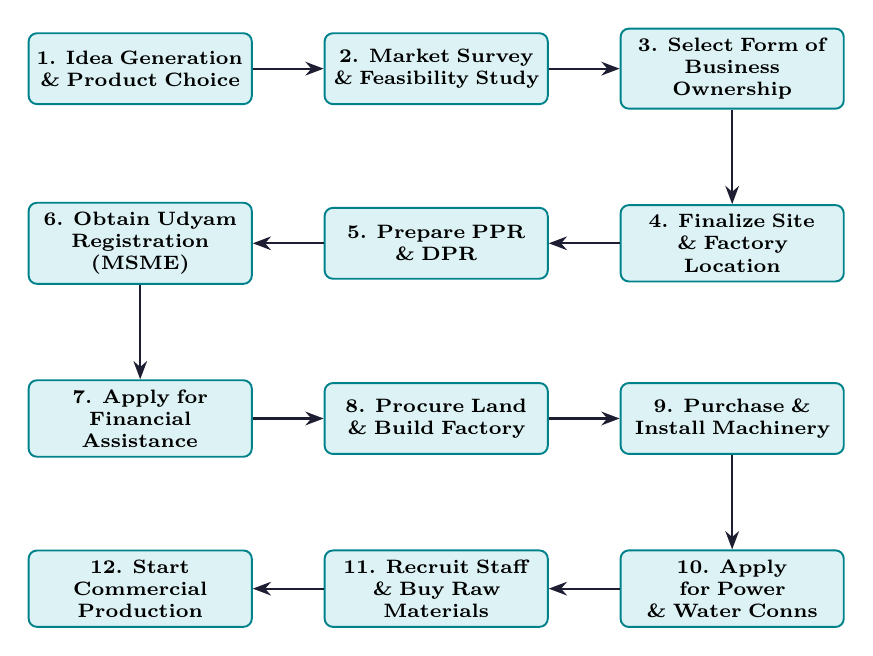
\begin{tikzpicture}[
  node distance=1.0cm and 0.9cm,
  block/.style={rectangle, draw=myteal, fill=hdrteal, text width=2.6cm, align=center, minimum height=0.9cm, font=\scriptsize\bfseries, rounded corners=3pt, line width=0.7pt},
  arrow/.style={-Stealth, thick, color=mydark}
]
  % Row 1
  \node[block] (s1) {1. Idea Generation \\ \& Product Choice};
  \node[block, right=of s1] (s2) {2. Market Survey \\ \& Feasibility Study};
  \node[block, right=of s2] (s3) {3. Select Form of \\ Business Ownership};
  
  % Row 2
  \node[block, below=1.2cm of s3] (s4) {4. Finalize Site \\ \& Factory Location};
  \node[block, left=of s4] (s5) {5. Prepare PPR \\ \& DPR};
  \node[block, left=of s5] (s6) {6. Obtain Udyam \\ Registration (MSME)};
  
  % Row 3
  \node[block, below=1.2cm of s6] (s7) {7. Apply for \\ Financial Assistance};
  \node[block, right=of s7] (s8) {8. Procure Land \\ \& Build Factory};
  \node[block, right=of s8] (s9) {9. Purchase \& \\ Install Machinery};
  
  % Row 4
  \node[block, below=1.2cm of s9] (s10) {10. Apply for Power \\ \& Water Conns};
  \node[block, left=of s10] (s11) {11. Recruit Staff \\ \& Buy Raw Materials};
  \node[block, left=of s11] (s12) {12. Start Commercial \\ Production};

  % Connective paths
  \draw[arrow] (s1) -- (s2);
  \draw[arrow] (s2) -- (s3);
  \draw[arrow] (s3) -- (s4);
  \draw[arrow] (s4) -- (s5);
  \draw[arrow] (s5) -- (s6);
  \draw[arrow] (s6) -- (s7);
  \draw[arrow] (s7) -- (s8);
  \draw[arrow] (s8) -- (s9);
  \draw[arrow] (s9) -- (s10);
  \draw[arrow] (s10) -- (s11);
  \draw[arrow] (s11) -- (s12);
\end{tikzpicture}
\end{tcolorbox}

\subsubsection{Details of the Process Steps}
\begin{enumerate}[label=\textbf{\arabic*.}, leftmargin=*, itemsep=3.5pt]
  \item \textbf{Idea Generation and Product Selection:} Identifying market demands or import substitutes. The entrepreneur selects a product based on their expertise, raw material availability, and market needs.
  \item \textbf{Market Survey and Feasibility Study:} Conducting surveys to estimate demand, competitive intensity, pricing points, and manufacturing costs.
  \item \textbf{Form of Business Ownership:} Deciding whether to register as a Sole Proprietorship, Partnership, Limited Liability Partnership (LLP), or a Private Limited Company.
  \item \textbf{Location and Site Selection:} Selecting a site with proximity to raw materials, labor, transport facilities, and markets, preferably in industrial estates.
  \item \textbf{Prepare PPR \& DPR:} Drafting a Preliminary Project Report (PPR) for initial clearances and a Detailed Project Report (DPR) to secure bank funding.
  \item \textbf{Udyam Registration:} Obtaining the official MSME registration online, which generates an Udyam Registration Number (URN).
  \item \textbf{Apply for Financing:} Submitting the DPR to banks or state financial corporations to secure term loans (for machinery) and working capital loans.
  \item \textbf{Land \& Building Development:} Registering land and constructing the factory layout according to local municipality and safety regulations.
  \item \textbf{Machinery and Equipment Procurement:} Ordering plant machinery from reliable vendors.
  \item \textbf{Utilities Connection:} Applying for industrial electrical power load from the state electricity board and water connections from the municipal board.
  \item \textbf{Workforce \& Material Procurement:} Recruiting technical staff and line workers, and placing orders for initial raw material batches.
  \item \textbf{Commercial Production:} Running trial batches to calibrate machinery and starting commercial manufacture.
\end{enumerate}

\newpage

% ===============================================================================
% MANDATORY QUICK REVISION PAGE
% ===============================================================================
\begin{center}
  {\large\bfseries\color{myred} Quick Revision --- Module 1}\\[3pt]
  {\small\color{mydark} Introduction \& Small Scale Industries $|$ OE-EC704C}
\end{center}
\noindent{\color{myred}\rule{\linewidth}{1.2pt}}
\vspace{4pt}

\begin{tcolorbox}[formulabox, title={\textbf{Key Concepts at a Glance}}]
\renewcommand{\arraystretch}{1.3}
\begin{tabularx}{\linewidth}{B{4.0cm} X}
NIP-91 & Liberalization, Privatization, and Globalization (LPG) reform model. \\
Composite Criteria 2020 & MSME classification combining Investment AND Turnover thresholds. \\
SSI (Small Enterprise) & Investment limit $\le \text{Rs. } 10 \text{ Crores}$ AND Annual Turnover $\le \text{Rs. } 50 \text{ Crores}$. \\
CGTMSE & Scheme offering collateral-free credit guarantee for MSME loans. \\
Udyam Portal & Paperless Aadhaar-linked registration system for Indian MSMEs. \\
n-Ach (Achievement Needs) & Key psychological driver of entrepreneurial risk-taking behavior. \\
\end{tabularx}
\end{tcolorbox}

\begin{tcolorbox}[defbox, title={\textbf{One-Line Definitions}}]
\begin{itemize}[leftmargin=*, itemsep=2.5pt, topsep=0pt]
  \item \textbf{Entrepreneurship:} Act of identifying business ideas, mobilizing capital, taking risk, and establishing a venture.
  \item \textbf{Intrapreneurship:} Act of driving innovation and new business lines within the safe environment of an established corporate firm.
  \item \textbf{Liberalization:} Deregulating industry by removing license limits and procedural bottlenecks.
  \item \textbf{Privatization:} Transferring ownership or operation of public enterprise assets to private ownership.
  \item \textbf{Small Scale Industry (SSI):} Enterprise with plant/machinery investment up to $10 \text{ Crores}$ and turnover up to $50 \text{ Crores}$.
  \item \textbf{District Industries Centre (DIC):} Centralized district-level agency providing support and licenses to local micro/small units.
  \item \textbf{Detailed Project Report (DPR):} Detailed feasibility plan and financial forecast document used to secure bank capital.
\end{itemize}
\end{tcolorbox}

\begin{tcolorbox}[exambox, title={\textbf{Frequently Asked / Viva Questions}}]
\begin{enumerate}[topsep=0pt, label=\textbf{Q\arabic*.}, itemsep=5pt]
  \item \Q{What were the main changes introduced in the Industrial Licensing policy of 1991?}
    Industrial licensing was completely abolished for all new projects, regardless of investment scale, except for five strategic or hazardous sectors (Defense, Explosives, Chemicals, Tobacco, Alcohol).
  \item \Q{How are Small Scale Industries defined post-2020 in India?}
    Under the 2020 composite criteria, a Small Enterprise (SSI) has an investment in plant/machinery of up to $\text{Rs. } 10\text{ Crores}$ and an annual turnover not exceeding $\text{Rs. } 50\text{ Crores}$.
  \item \Q{Differentiate between an Entrepreneur and an Intrapreneur.}
    An entrepreneur operates independently, mobilizes external capital, and bears all financial and personal risks. An intrapreneur behaves like an entrepreneur but works within a corporate system, utilizing corporate resources without personal financial exposure.
  \item \Q{State the contribution of SSIs to the Indian economy.}
    SSIs account for approximately 30\% of India's GDP, 45\% of total manufacturing output, and 40\% of direct/indirect exports, while being the second largest employer after agriculture.
  \item \Q{Identify the major causes for the dearth of entrepreneurial talent in India.}
    The major causes are socio-cultural stigma against business failure, a rote-learning oriented academic system that discourages critical thinking, limited access to early-stage collateral-free seed capital, and historical bureaucratic bottlenecks.
  \item \Q{What is the CGTMSE scheme?}
    The Credit Guarantee Fund Trust for Micro and Small Enterprises is a scheme that provides credit guarantees to commercial banks, allowing MSMEs to secure collateral-free loans up to $\text{Rs. } 2\text{ Crores}$.
  \item \Q{List the primary steps to start a Small Scale Industry.}
    Idea generation $\rightarrow$ Feasibility survey $\rightarrow$ Ownership structure $\rightarrow$ Location $\rightarrow$ PPR/DPR drafting $\rightarrow$ Udyam registration $\rightarrow$ Raising finance $\rightarrow$ Land/Factory development $\rightarrow$ Machine installation $\rightarrow$ Utility connections $\rightarrow$ Material procurement $\rightarrow$ Commercial production.
  \item \Q{What are District Industries Centres (DICs)?}
    DICs are district-level single-window clearance and support agencies that assist local entrepreneurs in obtaining licenses, raw material quotas, subsidies, and credit.
  \item \Q{Explain the MRTP Act change in NIP-91.}
    NIP-91 abolished the asset threshold limit of $\text{Rs. } 100\text{ Crores}$ for MRTP companies, allowing them to expand, merge, or establish new units without prior government approvals.
  \item \Q{What is FIPB and its purpose?}
    The Foreign Investment Promotion Board was established to process and approve foreign direct investment proposals in India that fell outside the automatic approval route.
  \end{enumerate}
\end{tcolorbox}


% -- Module 2 -----------------------------------------------------------------
\modulestart{2}{Market Survey and Research}

\section{Market Survey and Research}
% ===============================================================================

Before launching any product, an entrepreneur must understand consumer needs, market demand, and competitor behaviors. This is achieved through systematic market research and surveys.

\subsection{Market Survey vs. Market Research}
\begin{itemize}[leftmargin=*, itemsep=3pt]
  \item \textbf{Market Research:} A broad, systematic process of collecting, analyzing, and interpreting data about a market, including its size, segmentation, trends, competitors, and regulatory environment.
  \item \textbf{Market Survey:} A specific quantitative tool used within market research to gather structured opinions, feedback, or demographics from a representative sample of potential customers.
\end{itemize}

\subsection{Data Collection Methodologies}
\par\noindent
{\renewcommand{\arraystretch}{1.5}%
\begin{tabularx}{\linewidth}{|B{3.0cm}|Y|Y|}\hline
\multicolumn{1}{|>{\centering\arraybackslash}m{3.0cm}|}{\textbf{Feature}} &
\multicolumn{1}{>{\centering\arraybackslash}Y|}{\textbf{Primary Data}} &
\multicolumn{1}{>{\centering\arraybackslash}Y|}{\textbf{Secondary Data}} \\
\hline
\textbf{Definition} & Firsthand data collected directly for the specific research purpose. & Existing data gathered by third parties for other purposes. \\
\hline
\textbf{Methods} & Questionnaires, direct interviews, focus groups, observations. & Government census reports, industry journals, trade databases. \\
\hline
\textbf{Cost \& Time} & Highly expensive and time-consuming. & Relatively inexpensive and instantly accessible. \\
\hline
\textbf{Relevance} & 100\% tailored to the entrepreneur's immediate needs. & May be outdated, generic, or not fully aligned. \\
\hline
\textbf{Accuracy} & Controlled directly; high reliability. & Variable quality; requires validation. \\
\hline
\end{tabularx}
}

\subsection{Product Pricing Techniques}
Pricing directly determines sales velocity and profit margins. Entrepreneurs use several strategic pricing techniques:
\begin{enumerate}[label=\textbf{\arabic*.}, leftmargin=*, itemsep=4pt]
  \item \textbf{Cost-Plus Pricing (Markup Pricing):} The simplest method. A fixed percentage profit margin (markup) is added to the total cost of producing the product.
    \begin{equation}
      \text{Price} = \text{Unit Cost} \times (1 + \text{Markup Percentage})
    \end{equation}
  \item \textbf{Penetration Pricing:} Setting a very low initial price to attract a large volume of buyers quickly, establish market share, and discourage competitors. Prices are raised later once customer loyalty is secured.
  \item \textbf{Skimming Pricing:} Setting a high price initially for a new, innovative, or premium product to capture the maximum revenue from early adopters (who are less price-sensitive). Prices are lowered gradually to target broader segments.
  \item \textbf{Competitive Pricing:} Aligning the price directly with the prevailing market rates of close competitors, adjusting slightly for brand differentiation.
  \item \textbf{Demand-Based Pricing (Value-Based Pricing):} Setting prices primarily based on the perceived value to the consumer rather than the production cost (e.g., dynamic airline ticket pricing, premium software).
\end{enumerate}

% ===============================================================================
\section{Distribution Channels and Sales Promotion}
% ===============================================================================

\subsection{Distribution Channels}
\begin{tcolorbox}[defbox, title={Definition of Distribution Channel}]
A \textbf{Distribution Channel} (or marketing channel) is the pathway or chain of intermediaries (such as wholesalers, retailers, and agents) through which a product travels from the point of manufacture to the final consumer.
\end{tcolorbox}

\subsubsection{Types of Distribution Channels}
Distribution channels are classified based on the number of intermediary levels involved:

\begin{tcolorbox}[tikzbox, title={Structure of Distribution Channels}]
\centering
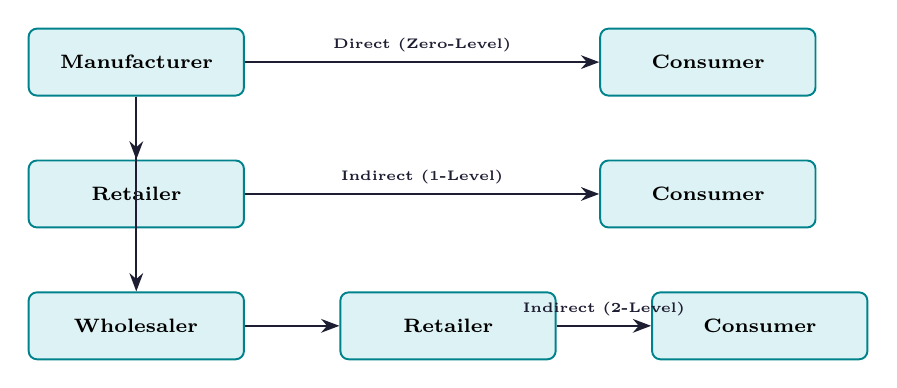
\begin{tikzpicture}[
  node distance=0.8cm and 1.2cm,
  block/.style={rectangle, draw=myteal, fill=hdrteal, text width=2.5cm, align=center, minimum height=0.85cm, font=\scriptsize\bfseries, rounded corners=3pt, line width=0.7pt},
  arrow/.style={-Stealth, thick, color=mydark}
]
  \node[block] (m) {Manufacturer};
  
  % Level 0
  \node[block, right=4.5cm of m] (c1) {Consumer};
  \draw[arrow] (m) -- node[above, font=\tiny\bfseries\color{myred}] {Direct (Zero-Level)} (c1);
  
  % Level 1
  \node[block, below=of m] (r) {Retailer};
  \node[block, right=4.5cm of r] (c2) {Consumer};
  \draw[arrow] (m) -- (r);
  \draw[arrow] (r) -- node[above, font=\tiny\bfseries\color{myteal}] {Indirect (1-Level)} (c2);
  
  % Level 2
  \node[block, below=of r] (w) {Wholesaler};
  \node[block, right=of w] (r2) {Retailer};
  \node[block, right=of r2] (c3) {Consumer};
  \draw[arrow] (m) -- (w);
  \draw[arrow] (w) -- (r2);
  \draw[arrow] (r2) -- node[above, font=\tiny\bfseries\color{myamber}] {Indirect (2-Level)} (c3);
\end{tikzpicture}
\end{tcolorbox}

\subsubsection{Factors Influencing Channel Selection}
An entrepreneur must select channels based on four critical factors:
\begin{itemize}[leftmargin=*, itemsep=3pt]
  \item \textbf{Product Characteristics:} Perishable goods (e.g., food) require direct/short channels. Industrial, high-value, or customized items (e.g., machinery) also use direct sales, while standardized, durable consumer goods use multi-level channels.
  \item \textbf{Market Factors:} A scattered consumer base requires wholesalers and retailers. If the target market is small and concentrated, direct selling is optimal.
  \item \textbf{Company Resources:} Startups with limited capital and sales force rely on existing distributor networks. Strong companies can establish direct retail outlets.
  \item \textbf{Middlemen Capability:} Availability of reliable distributors, credit-worthiness, and the margin share they demand.
\end{itemize}

\subsection{Sales Promotion Activities}
Sales promotion includes short-term incentives to encourage quick purchases of a product.
\begin{itemize}[leftmargin=*, itemsep=3.5pt]
  \item \textbf{Consumer-Oriented Promotions:} Target the end customer directly.
    \begin{itemize}[label=\tiny$\bullet$, leftmargin=1.5em, itemsep=2pt]
      \item \textit{Price Discounts \& Rebates:} Temporary price cuts (e.g., 20\% off, ``Buy 1 Get 1 Free'').
      \item \textit{Coupons:} Certificates offering a specified discount on purchase.
      \item \textit{Free Samples:} Distributing small quantities of the product to encourage trial.
      \item \textit{Contests/Sweepstakes:} Competitions where buyers stand a chance to win prizes.
    \end{itemize}
  \item \textbf{Trade-Oriented Promotions:} Target intermediaries (distributors, retailers) to push the product.
    \begin{itemize}[label=\tiny$\bullet$, leftmargin=1.5em, itemsep=2pt]
      \item \textit{Trade Allowances:} Financial incentives/discounts for stocking and displaying products.
      \item \textit{Cooperative Advertising:} Manufacturer shares local advertising costs with the retailer.
      \item \textit{Dealer Sales Contests:} Rewarding dealers who achieve peak sales volumes.
    \end{itemize}
\end{itemize}

% ===============================================================================
\section{Raising Business Finance}
% ===============================================================================

Capital is the lifeblood of any enterprise. Financing is categorized into Equity (ownership capital) and Debt (borrowed capital).

\subsection{Debt vs. Equity Financing}
\par\noindent
{\renewcommand{\arraystretch}{1.5}%
\begin{tabularx}{\linewidth}{|B{2.8cm}|Y|Y|}\hline
\multicolumn{1}{|>{\centering\arraybackslash}m{2.8cm}|}{\textbf{Parameter}} &
\multicolumn{1}{>{\centering\arraybackslash}Y|}{\textbf{Equity Financing}} &
\multicolumn{1}{>{\centering\arraybackslash}Y|}{\textbf{Debt Financing}} \\
\hline
\textbf{Ownership} & Dilutes ownership; investors get voting rights and shares. & No dilution of ownership; lender has no say in management. \\
\hline
\textbf{Repayment} & No obligation to repay; profits are distributed as dividends. & Legal obligation to make regular principal and interest payments. \\
\hline
\textbf{Collateral} & No collateral or asset pledge required. & Often requires tangible assets or personal guarantees. \\
\hline
\textbf{Cost} & High cost in the long run (giving away future profits). & Lower cost (fixed interest rate, which is tax-deductible). \\
\hline
\textbf{Risk} & Zero bankruptcy risk; safe for early-stage ventures. & High risk; default can lead to asset foreclosure and insolvency. \\
\hline
\end{tabularx}
}

\subsection{Sources of Startup Finance}
\begin{enumerate}[label=\textbf{\arabic*.}, leftmargin=*, itemsep=4pt]
  \item \textbf{Bootstrapping (Self-Funding):} The entrepreneur uses personal savings, credit cards, or loans from friends/family. It retains 100\% equity but limits growth scope.
  \item \textbf{Angel Investors:} Wealthy individuals who invest their personal capital in early-stage startups in exchange for equity. They also provide mentorship and networks.
  \item \textbf{Venture Capital (VC):} Professional firms that manage pooled funds from institutional investors to invest in high-growth, scalable startups. They invest larger tickets during Series A, B, etc., and demand board seats.
  \item \textbf{Commercial Banks \& Financial Institutions:} Conventional term loans or lines of credit. Suitable for asset acquisition (machinery/land) once the business has cash flow.
  \item \textbf{Government Initiatives (India):}
    \begin{itemize}[label=\tiny$\bullet$, leftmargin=1.5em, itemsep=2pt]
      \item \textit{MUDRA Loans (PMMY):} Low-interest loans up to $\text{Rs. } 10 \text{ Lakhs}$ under Shishu, Kishor, and Tarun schemes for micro-enterprises.
      \item \textit{Startup India Seed Fund Scheme (SISFS):} Provides grants/loans to startups for proof of concept, prototype development, and market entry.
    \end{itemize}
\end{enumerate}

% ===============================================================================
\section{Enterprise Launching Formalities}
% ===============================================================================

Once the finance is secured and the product is finalized, the entrepreneur must complete the legal launching process:

\subsection{Legal Formality Checklist}
\begin{itemize}[leftmargin=*, itemsep=3.5pt]
  \item \textbf{Entity Registration:} Register the business name and structure (Ministry of Corporate Affairs for Private Ltd/LLP, or local Registrar of Firms for Partnership).
  \item \textbf{Tax Registrations:}
    \begin{itemize}[label=\tiny$\bullet$, leftmargin=1.5em, itemsep=2.0pt]
      \item \textit{Permanent Account Number (PAN):} Required for all corporate banking and tax filings.
      \item \textit{GSTIN Registration:} Mandatory for businesses with inter-state sales or annual turnover exceeding the threshold ($\text{Rs. } 40 \text{ Lakhs}$ for goods / $\text{Rs. } 20 \text{ Lakhs}$ for services).
    \end{itemize}
  \item \textbf{Municipal/Local Licenses:} Trade License from the local Municipal Corporation, and Shops and Establishment Act registration.
  \item \textbf{Environmental and Safety Approvals:} Consent to Establish (CTE) and Consent to Operate (CTO) from the State Pollution Control Board (SPCB) for manufacturing units. Fire safety clearance.
  \item \textbf{Udyam (MSME) Registration:} Completed online for benefits under government procurement and priority lending schemes.
  \item \textbf{Commercial Bank Account:} Opening a current account in the name of the registered entity to keep business transactions separate.
\end{itemize}

\newpage

% ===============================================================================
% MANDATORY QUICK REVISION PAGE
% ===============================================================================
\begin{center}
  {\large\bfseries\color{myred} Quick Revision --- Module 2}\\[3pt]
  {\small\color{mydark} Marketing, Financing \& Launching $|$ OE-EC704C}
\end{center}
\noindent{\color{myred}\rule{\linewidth}{1.2pt}}
\vspace{4pt}

\begin{tcolorbox}[formulabox, title={\textbf{Key Concepts at a Glance}}]
\renewcommand{\arraystretch}{1.3}
\begin{tabularx}{\linewidth}{B{4.0cm} X}
Primary Data & Firsthand market feedback (custom, expensive, accurate). \\
Skimming Pricing & High initial price for innovative products $\rightarrow$ lower gradually. \\
Penetration Pricing & Low initial price to capture market share $\rightarrow$ raise later. \\
Markup Formula & $\text{Selling Price} = \text{Unit Cost} \times (1 + \text{Markup \%})$. \\
Zero-Level Channel & Direct path: $\text{Manufacturer} \rightarrow \text{Consumer}$ (no middlemen). \\
Angel Investors & Wealthy individuals investing personal money in early-stage startups. \\
GSTIN & 15-digit unique Goods and Services Tax Identification Number. \\
\end{tabularx}
\end{tcolorbox}

\begin{tcolorbox}[defbox, title={\textbf{One-Line Definitions}}]
\begin{itemize}[leftmargin=*, itemsep=2.5pt, topsep=0pt]
  \item \textbf{Market Research:} Systematic process of gathering and analyzing data about a target market and its competitors.
  \item \textbf{Value-Based Pricing:} Setting price based on the customer's perceived value rather than production cost.
  \item \textbf{Distribution Channel:} Chain of businesses or intermediaries through which a product passes to the final buyer.
  \item \textbf{Sales Promotion:} Short-term incentives designed to stimulate immediate demand and sales.
  \item \textbf{Equity Financing:} Raising capital by selling shares of ownership in the company.
  \item \textbf{Debt Financing:} Borrowing capital that must be repaid over time with interest.
  \item \textbf{Venture Capital:} Funds invested in high-risk, high-growth startups by professional firms.
\end{itemize}
\end{tcolorbox}

\begin{tcolorbox}[exambox, title={\textbf{Frequently Asked / Viva Questions}}]
\begin{enumerate}[topsep=0pt, label=\textbf{Q\arabic*.}, itemsep=5pt]
  \item \Q{Compare primary data and secondary data in market surveys.}
    Primary data is collected firsthand for the specific study (e.g., questionnaires) and is highly relevant but expensive. Secondary data already exists (e.g., government reports) and is cheap and fast but might be generic or outdated.
  \item \Q{When is Skimming Pricing used instead of Penetration Pricing?}
    Skimming is used for highly innovative, patented, or luxury products to recover development costs from early adopters. Penetration is used in highly competitive markets to capture rapid volume and build a barrier for rivals.
  \item \Q{What is a Zero-Level distribution channel? Give an example.}
    It is a direct channel where the manufacturer sells directly to the consumer without any intermediaries. Examples: factory outlets, e-commerce websites, and door-to-door sales.
  \item \Q{What factors dictate the selection of a distribution channel?}
    Product characteristics (perishability, value), market characteristics (customer density, geography), company resources (budget, sales force), and middlemen capabilities (margins, reach).
  \item \Q{Differentiate between consumer promotion and trade promotion.}
    Consumer promotion targets the end-user (e.g., coupons, free samples) to pull products off shelves. Trade promotion targets wholesalers/retailers (e.g., display allowances, trade discounts) to push products through the channel.
  \item \Q{Why is debt financing considered cheaper than equity financing in the long run?}
    Interest payments on debt are fixed and tax-deductible, and debt does not dilute ownership or future profits. Equity dilute ownership permanently, making it expensive if the company grows highly profitable.
  \item \Q{Define Venture Capital (VC).}
    Venture Capital is professional private equity investment provided to early-stage, high-potential startups with high growth scalability, in exchange for equity and significant managerial influence.
  \item \Q{What is the purpose of Udyam registration for a launching startup?}
    It provides MSME classification, which unlocks interest rate concessions on bank loans, collateral-free credit guarantees, subsidies on patents, and eligibility for government procurement tenders.
  \item \Q{What are the mandatory tax registrations required to start commercial sales in India?}
    Permanent Account Number (PAN) for income tax and financial transactions, and Goods and Services Tax Identification Number (GSTIN) for indirect tax compliance.
  \item \Q{Name two government financing schemes for MSMEs in India.}
    The MUDRA Yojana (PMMY) for micro-loans up to $\text{Rs. } 10 \text{ Lakhs}$, and the Startup India Seed Fund Scheme (SISFS) for early-stage proof-of-concept capital.
  \end{enumerate}
\end{tcolorbox}


% -- Module 3 -----------------------------------------------------------------
\modulestart{3}{Financial Management \& Working Capital}

\section{Financial Management \& Working Capital}
% ===============================================================================

\subsection{Financial Management Goals}
Financial management involves the planning, organizing, and controlling of financial resources to meet business objectives. There are two primary goals:
\begin{itemize}[leftmargin=*, itemsep=3.5pt]
  \item \textbf{Profit Maximization:} Focuses on increasing the net profit of the firm in the short term.
    \textit{Limitations:} Ignores the time value of money, ignores risks and uncertainty, and can lead to short-sighted decision-making.
  \item \textbf{Wealth Maximization (Value Maximization):} Focuses on maximizing the market value of the company's shares.
    \textit{Advantages:} Considers the time value of money, accounts for risk, and aims at long-term sustainable growth for shareholders.
\end{itemize}

\subsection{Working Capital Management}
Working capital represents the funds required to finance the day-to-day operations of an enterprise.

\begin{tcolorbox}[defbox, title={Working Capital Concepts}]
\begin{itemize}[leftmargin=*, itemsep=2.2pt, topsep=0pt]
  \item \textbf{Gross Working Capital:} Total investment in current assets (Cash + Receivables + Inventory + Short-Term Securities).
  \item \textbf{Net Working Capital:} Current Assets minus Current Liabilities. This represents the long-term funds financing current assets.
    \begin{equation}
      \text{NWC} = \text{Current Assets (CA)} - \text{Current Liabilities (CL)}
    \end{equation}
\end{itemize}
\end{tcolorbox}

\subsubsection{The Operating Cycle (Working Capital Cycle)}
The operating cycle is the duration of time required to convert raw materials back into cash through sales.

\begin{tcolorbox}[formulabox, title={Operating Cycle Length Calculation}]
The length of the Operating Cycle ($O$) in days is calculated as:
\begin{equation}
  O = R + W + F + D - C
\end{equation}
Where:
\begin{align*}
  R &= \text{Raw Material Storage Period} = \frac{\text{Average Stock of Raw Materials}}{\text{Daily Raw Material Consumption}} \\
  W &= \text{Work-in-Progress (WIP) Conversion Period} = \frac{\text{Average Stock of WIP}}{\text{Daily Cost of Production}} \\
  F &= \text{Finished Goods Storage Period} = \frac{\text{Average Stock of Finished Goods}}{\text{Daily Cost of Sales}} \\
  D &= \text{Debtors (Accounts Receivable) Collection Period} = \frac{\text{Average Accounts Receivable}}{\text{Daily Credit Sales}} \\
  C &= \text{Creditors (Accounts Payable) Payment Period} = \frac{\text{Average Accounts Payable}}{\text{Daily Credit Purchases}}
\end{align*}
\end{tcolorbox}

% ===============================================================================
\section{Costing and Book Keeping}
% ===============================================================================

\subsection{Elements of Cost}
Cost is divided into three primary categories to assist in pricing and control:
\begin{enumerate}[label=\textbf{\arabic*.}, leftmargin=*, itemsep=3pt]
  \item \textbf{Material Cost:} Cost of substances from which the product is manufactured.
    \begin{itemize}[label=\tiny$\bullet$, leftmargin=1.5em, itemsep=1.5pt]
      \item \textit{Direct Material:} Identifiable in the final product (e.g., steel in a car).
      \item \textit{Indirect Material:} Auxiliary items (e.g., lubricants, cleaning rags).
    \end{itemize}
  \item \textbf{Labour Cost:} Cost of wages paid to employees.
    \begin{itemize}[label=\tiny$\bullet$, leftmargin=1.5em, itemsep=1.5pt]
      \item \textit{Direct Labour:} Hands-on production staff (e.g., assembly line workers).
      \item \textit{Indirect Labour:} Supportive staff (e.g., supervisors, security).
    \end{itemize}
  \item \textbf{Expenses:} Cost of services other than materials and labor.
    \begin{itemize}[label=\tiny$\bullet$, leftmargin=1.5em, itemsep=1.5pt]
      \item \textit{Direct Expenses:} Hire charges for special tools for a specific job.
      \item \textit{Indirect Expenses (Overheads):} Rent, power, insurance, depreciation.
    \end{itemize}
\end{enumerate}

\subsection{Book Keeping Systems}
Bookkeeping is the recording phase of financial accounting.
\begin{itemize}[leftmargin=*, itemsep=3.5pt]
  \item \textbf{Single-Entry System:} An incomplete, informal system where only personal accounts and cash book records are maintained. It is prone to errors and cannot generate a balance sheet.
  \item \textbf{Double-Entry System:} A scientific, comprehensive system where every transaction affects at least two accounts (one debit, one credit) in opposite directions:
    \begin{equation}
      \text{Assets} = \text{Liabilities} + \text{Owner's Equity}
    \end{equation}
\end{itemize}

\subsubsection{Double-Entry Golden Rules of Accounting}
\par\noindent
{\renewcommand{\arraystretch}{1.5}%
\begin{tabularx}{\linewidth}{|B{3.0cm}|Y|Y|}\hline
\multicolumn{1}{|>{\centering\arraybackslash}m{3.0cm}|}{\textbf{Account Type}} &
\multicolumn{1}{>{\centering\arraybackslash}Y|}{\textbf{Debit Rules (Dr.)}} &
\multicolumn{1}{>{\centering\arraybackslash}Y|}{\textbf{Credit Rules (Cr.)}} \\
\hline
Real Account (Assets) & Debit what comes in. & Credit what goes out. \\
\hline
Personal Account (People/Firms) & Debit the receiver. & Credit the giver. \\
\hline
Nominal Account (Expenses/Gains) & Debit all expenses and losses. & Credit all incomes and gains. \\
\hline
\end{tabularx}
}

\subsubsection{Accounting Process Flow}
$$\text{Source Documents} \rightarrow \text{Journal (Day Book)} \rightarrow \text{Ledger (T-Accounts)} \rightarrow \text{Trial Balance} \rightarrow \text{Final Accounts}$$

% ===============================================================================
\section{Break-Even Analysis}
% ===============================================================================

Break-even analysis is a financial tool used to determine the level of output or sales volume at which a business earns zero profit and suffers zero loss.

\subsection{Mathematical Derivation of BEP}
Let:
\begin{align*}
  S &= \text{Selling Price per Unit} \\
  V &= \text{Variable Cost per Unit} \\
  F &= \text{Total Fixed Cost} \\
  Q &= \text{Quantity of Units Sold} \\
  R &= \text{Total Sales Revenue} = S \times Q \\
  TC &= \text{Total Cost} = F + (V \times Q) \\
  P &= \text{Net Profit} = R - TC = (S \times Q) - [F + (V \times Q)]
\end{align*}
At the \textbf{Break-Even Point (BEP)}, Profit ($P$) is zero:
\begin{equation*}
  (S \times Q_{BEP}) - F - (V \times Q_{BEP}) = 0
\end{equation*}
\begin{equation*}
  Q_{BEP} (S - V) = F
\end{equation*}
\begin{equation}
  Q_{BEP} \text{ (in Units)} = \frac{F}{S - V} = \frac{\text{Fixed Cost}}{\text{Contribution per Unit}}
\end{equation}
To find the Break-Even Sales value ($S_{BEP}$ in Rupees):
\begin{equation}
  S_{BEP} \text{ (in Rs.)} = Q_{BEP} \times S = \frac{F \times S}{S - V} = \frac{F}{1 - \frac{V}{S}} = \frac{\text{Fixed Cost}}{\text{P/V Ratio}}
\end{equation}

\subsection{Profit-Volume (P/V) Ratio \& Margin of Safety}
\begin{tcolorbox}[formulabox, title={P/V Ratio and Margin of Safety Formulas}]
\begin{itemize}[leftmargin=*, itemsep=3.5pt, topsep=0pt]
  \item \textbf{P/V Ratio (Contribution Margin Ratio):}
    \begin{equation}
      \text{P/V Ratio} = \frac{\text{Contribution}}{\text{Sales}} = \frac{S - V}{S} = \frac{\text{Fixed Cost} + \text{Profit}}{\text{Sales}}
    \end{equation}
  \item \textbf{Margin of Safety (MoS):} The excess of actual/planned sales over the break-even sales. It represents the cushion against sales drop before incurring a loss.
    \begin{equation}
      \text{MoS (in Units)} = \text{Actual Sales (Units)} - Q_{BEP}
    \end{equation}
    \begin{equation}
      \text{MoS (in Rs.)} = \text{Actual Sales Value} - S_{BEP} = \frac{\text{Profit}}{\text{P/V Ratio}}
    \end{equation}
    \begin{equation}
      \text{MoS Percentage} = \frac{\text{Actual Sales} - \text{BEP Sales}}{\text{Actual Sales}} \times 100\%
    \end{equation}
\end{itemize}
\end{tcolorbox}

\subsection{The Break-Even Chart}
The graphical representation of cost, volume, and profit relationships:

\begin{tcolorbox}[tikzbox, title={The Break-Even Chart}]
\centering
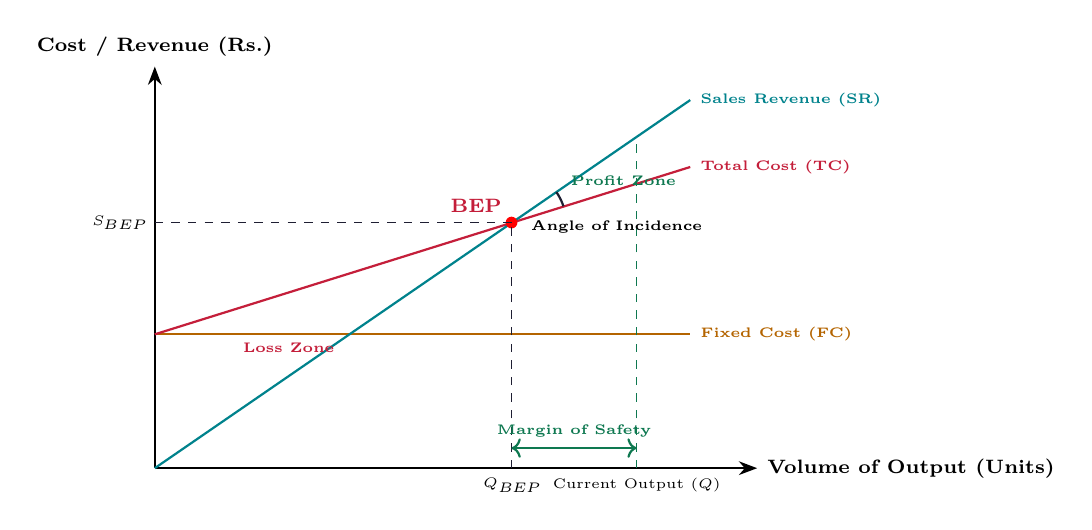
\begin{tikzpicture}[scale=0.85]
  % Draw Axes
  \draw[-Stealth, thick] (0,0) -- (9,0) node[right, font=\scriptsize\bfseries] {Volume of Output (Units)};
  \draw[-Stealth, thick] (0,0) -- (0,6) node[above, font=\scriptsize\bfseries] {Cost / Revenue (Rs.)};
  
  % Fixed Cost Line
  \draw[thick, color=myamber] (0,2) -- (8,2) node[right, font=\tiny\bfseries] {Fixed Cost (FC)};
  
  % Total Cost Line
  \draw[thick, color=myred] (0,2) -- (8,4.5) node[right, font=\tiny\bfseries] {Total Cost (TC)};
  
  % Sales Revenue Line
  \draw[thick, color=myteal] (0,0) -- (8,5.5) node[right, font=\tiny\bfseries] {Sales Revenue (SR)};
  
  % Break-Even Point Intersection
  % (5.5/8)*x = 2 + (2.5/8)*x => (3/8)*x = 2 => x = 16/3 = 5.33
  % y = (5.5/8)*5.33 = 3.67
  \coordinate (BEP) at (5.33,3.67);
  \fill[red] (BEP) circle (2.5pt);
  \node[above left, font=\scriptsize\bfseries, color=myred] at (BEP) {BEP};
  
  % Dashed projections from BEP
  \draw[dashed, color=mydark] (5.33,0) -- (5.33,3.67);
  \draw[dashed, color=mydark] (0,3.67) -- (5.33,3.67);
  \node[below, font=\tiny] at (5.33,0) {$Q_{BEP}$};
  \node[left, font=\tiny] at (0,3.67) {$S_{BEP}$};
  
  % Current output level projection
  \draw[dashed, color=mygreen] (7.2,0) -- (7.2,4.95);
  \node[below, font=\tiny] at (7.2,0) {Current Output ($Q$)};
  
  % Margin of Safety indicator
  \draw[<->, thick, color=mygreen] (5.33,0.3) -- (7.2,0.3) node[midway, above, font=\tiny\bfseries] {Margin of Safety};
  
  % Loss and Profit Zones
  \node[font=\tiny\bfseries, color=myred] at (2,1.8) {Loss Zone};
  \node[font=\tiny\bfseries, color=mygreen] at (7,4.3) {Profit Zone};
  
  % Angle of Incidence
  \draw[thick, color=mydark] (6.0,4.125) arc (35:18:0.8);
  \node[font=\tiny\bfseries] at (6.9,3.6) {Angle of Incidence};
\end{tikzpicture}
\end{tcolorbox}

% ===============================================================================
\section{Overview of Taxation}
% ===============================================================================

Taxes are compulsory levies by governments on individuals or corporations.

\subsection{Direct vs. Indirect Taxes}
\begin{itemize}[leftmargin=*, itemsep=3.5pt]
  \item \textbf{Direct Tax:} A tax levied directly on the income or wealth of a person or corporation (e.g., \textbf{Income Tax}). The burden of this tax cannot be shifted to another person.
  \item \textbf{Indirect Tax:} A tax levied on goods and services (e.g., \textbf{Excise Duty, Sales Tax, VAT, GST}). The burden is shifted to the final consumer in the form of higher prices.
\end{itemize}

\subsection{Traditional Indirect Tax Elements}
Before the implementation of GST (2017) in India, the indirect tax structure consisted of:
\begin{enumerate}[label=\textbf{\alph*.}, leftmargin=*, itemsep=2.5pt]
  \item \textbf{Excise Duty:} Tax levied on the manufacture/production of goods within the country.
  \item \textbf{Sales Tax:} Tax levied on the transfer of ownership of goods (intrastate or interstate).
  \item \textbf{Value Added Tax (VAT):} A multi-stage tax levied on the value added at each stage of production and distribution, allowing credit for tax paid on inputs (Input Tax Credit), which minimized cascading tax effects.
\end{enumerate}

\newpage

% ===============================================================================
% MANDATORY QUICK REVISION PAGE
% ===============================================================================
\begin{center}
  {\large\bfseries\color{myred} Quick Revision --- Module 3}\\[3pt]
  {\small\color{mydark} Accounting, BEP \& Taxation $|$ OE-EC704C}
\end{center}
\noindent{\color{myred}\rule{\linewidth}{1.2pt}}
\vspace{4pt}

\begin{tcolorbox}[formulabox, title={\textbf{Key Concepts \& Equations}}]
\renewcommand{\arraystretch}{1.4}
\begin{tabularx}{\linewidth}{B{4.0cm} X}
Net Working Capital & $\text{NWC} = \text{Current Assets} - \text{Current Liabilities}$. \\
Operating Cycle & $O = R + W + F + D - C$ (days). \\
BEP (Units) & $Q_{BEP} = \frac{\text{Fixed Cost}}{\text{Selling Price} - \text{Variable Cost}} = \frac{F}{S - V}$. \\
P/V Ratio & $\text{P/V} = \frac{\text{Contribution}}{\text{Sales}} = \frac{S - V}{S}$. \\
BEP (Rupees) & $S_{BEP} = \frac{\text{Fixed Cost}}{\text{P/V Ratio}}$. \\
Margin of Safety (MoS) & $\text{MoS (Rs.)} = \text{Actual Sales Value} - S_{BEP} = \frac{\text{Profit}}{\text{P/V Ratio}}$. \\
Accounting Equation & $\text{Assets} = \text{Liabilities} + \text{Capital}$. \\
\end{tabularx}
\end{tcolorbox}

\begin{tcolorbox}[defbox, title={\textbf{One-Line Definitions}}]
\begin{itemize}[leftmargin=*, itemsep=2.5pt, topsep=0pt]
  \item \textbf{Wealth Maximization:} Maximizing the long-term stock value of a company.
  \item \textbf{Operating Cycle:} Time taken from cash investment in raw materials to cash collection from buyers.
  \item \textbf{Nominal Accounts:} Accounts recording business expenses, losses, incomes, and gains.
  \item \textbf{Contribution:} Excess of sales revenue over variable costs ($S - V$).
  \item \textbf{Angle of Incidence:} The angle formed between the sales line and total cost line on a BEP chart; larger angles indicate faster profit generation.
  \item \textbf{Direct Tax:} Tax paid directly to the government by the earner (burden cannot be shifted).
  \item \textbf{VAT:} Multi-stage tax on goods where tax paid on inputs is credited.
\end{itemize}
\end{tcolorbox}

\begin{tcolorbox}[exambox, title={\textbf{Frequently Asked / Viva Questions}}]
\begin{enumerate}[topsep=0pt, label=\textbf{Q\arabic*.}, itemsep=5pt]
  \item \Q{Compare Profit Maximization and Wealth Maximization.}
    Profit Maximization is short-term and ignores risk and the time value of money. Wealth Maximization is a long-term goal that maximizes the market value of company shares, taking risk and timing of cash flows into account.
  \item \Q{What is the effect of increasing the credit period allowed to debtors on working capital?}
    Increasing the debtor credit period ($D$) lengthens the operating cycle, keeping capital tied up longer and increasing the working capital requirement.
  \item \Q{State the golden rule of real accounts.}
    Debit what comes in (increase in assets); Credit what goes out (decrease in assets).
  \item \Q{List the elements of cost in a manufacturing unit.}
    Cost of Materials (Direct and Indirect), Cost of Labour (Direct and Indirect), and Expenses/Overheads (Direct and Indirect).
  \item \Q{Differentiate between Journal and Ledger.}
    A journal is the book of prime entry where transactions are recorded chronologically. A ledger is the principal book where journal entries are classified and posted into individual accounts (T-accounts).
  \item \Q{What are the key assumptions in Break-Even Analysis?}
    Assumptions: All costs can be split into fixed and variable components; Fixed costs remain constant; Variable cost per unit remains constant; Selling price per unit remains constant; Sales volume equals production volume.
  \item \Q{What does a high Margin of Safety (MoS) indicate?}
    A high MoS indicates that the business is highly profitable and can withstand a significant decline in sales volume before hitting the break-even threshold and incurring losses.
  \item \Q{How does the Angle of Incidence affect profit capacity?}
    A large Angle of Incidence indicates a steep sales revenue line relative to total costs. It shows that the firm generates profits rapidly once the break-even point is passed.
  \item \Q{Differentiate between Direct and Indirect taxes with examples.}
    Direct tax (e.g., Income Tax) is levied on income and the burden cannot be shifted. Indirect tax (e.g., GST or Excise Duty) is levied on goods and services, and the cost burden is shifted to the final consumer.
  \item \Q{What is Input Tax Credit (ITC) under VAT?}
    ITC allows a manufacturer or seller to deduct the tax already paid on purchases (inputs) from the tax liability on sales (outputs), avoiding double taxation on the same product.
  \end{enumerate}
\end{tcolorbox}


% -- Module 4 -----------------------------------------------------------------
\modulestart{4}{Decision Making in Management}

\section{Decision Making in Management}
% ===============================================================================

\subsection{Meaning and Types of Decisions}
\begin{tcolorbox}[defbox, title={Definition of Decision Making}]
\textbf{Decision Making} is the cognitive process of identifying and selecting a course of action from among several alternatives to solve a specific problem or achieve a desired organizational goal.
\end{tcolorbox}

Managers classify decisions into several core topologies:
\begin{itemize}[leftmargin=*, itemsep=3.5pt]
  \item \textbf{Programmed vs. Non-Programmed Decisions:}
    \begin{itemize}[label=\tiny$\bullet$, leftmargin=1.5em, itemsep=1.5pt]
      \item \textit{Programmed:} Routine, repetitive decisions handled through established rules, policies, or procedures (e.g., reordering inventory when it hits a reorder level).
      \item \textit{Non-Programmed:} Unique, unstructured, and complex decisions requiring custom problem-solving, strategic judgment, and creative thinking (e.g., launching a new product line).
    \end{itemize}
  \item \textbf{Strategic vs. Operational Decisions:}
    \begin{itemize}[label=\tiny$\bullet$, leftmargin=1.5em, itemsep=1.5pt]
      \item \textit{Strategic:} High-stake, long-term decisions made by top management affecting the entire organization (e.g., expanding into international markets).
      \item \textit{Operational:} Short-term, day-to-day decisions made by lower-level managers to ensure smooth daily processes (e.g., scheduling worker shifts).
    \end{itemize}
\end{itemize}

\subsection{The Rational Decision-Making Process}
Rational decision-making involves 7 sequential steps:
$$\text{Identify Problem} \rightarrow \text{Gather Info} \rightarrow \text{Develop Alternatives} \rightarrow \text{Evaluate Options} \rightarrow \text{Select Choice} \rightarrow \text{Implement} \rightarrow \text{Review \& Feedback}$$

% ===============================================================================
\section{Forecasting Methodologies}
% ===============================================================================

Forecasting is the process of predicting future events or demands based on historical data and analytical models. It is critical for planning production, inventory, and finances.

\subsection{Qualitative vs. Quantitative Forecasting}
\par\noindent
{\renewcommand{\arraystretch}{1.5}%
\begin{tabularx}{\linewidth}{|B{3.0cm}|Y|Y|}\hline
\multicolumn{1}{|>{\centering\arraybackslash}m{3.0cm}|}{\textbf{Feature}} &
\multicolumn{1}{>{\centering\arraybackslash}Y|}{\textbf{Qualitative Methods}} &
\multicolumn{1}{>{\centering\arraybackslash}Y|}{\textbf{Quantitative Methods}} \\
\hline
\textbf{Basis} & Subjective judgment, intuition, and expert opinions. & Mathematical models and historical numerical data. \\
\hline
\textbf{Context} & Used when historical data is unavailable (e.g., new products). & Used when stable historical data is available (e.g., mature products). \\
\hline
\textbf{Key Techniques} & Delphi method, Jury of Executive Opinion, Sales Force Composite. & Time-Series models (moving averages, exponential smoothing), Regression models. \\
\hline
\textbf{Cost \& Accuracy} & Highly subjective; variable long-term accuracy. & Highly objective; reliable short-term mathematical accuracy. \\
\hline
\end{tabularx}
}

\subsection{Key Forecasting Techniques}
\begin{itemize}[leftmargin=*, itemsep=3.5pt]
  \item \textbf{Delphi Method (Qualitative):} A structured communication technique where a panel of experts answers questionnaires in two or more rounds. After each round, a facilitator provides an anonymous summary of the experts' forecasts and reasons. Experts are encouraged to revise their earlier answers, converging toward a consensus.
  \item \textbf{Simple Moving Average (Quantitative):} Predicts demand for the next period ($F_{t+1}$) by averaging the actual demand ($A_t$) over a fixed number of past periods ($n$):
    \begin{equation}
      F_{t+1} = \frac{A_t + A_{t-1} + \dots + A_{t-n+1}}{n}
    \end{equation}
  \item \textbf{Exponential Smoothing (Quantitative):} A weighted moving average method where recent data is weighted more heavily. The forecast ($F_{t+1}$) is calculated using the smoothing constant $\alpha$ ($0 \le \alpha \le 1$):
    \begin{equation}
      F_{t+1} = F_t + \alpha (A_t - F_t) = \alpha A_t + (1 - \alpha) F_t
    \end{equation}
\end{itemize}

% ===============================================================================
\section{Personnel Management}
% ===============================================================================

\subsection{Meaning and Core Functions}
\begin{tcolorbox}[defbox, title={Definition of Personnel Management}]
\textbf{Personnel Management} (often structured as Human Resource Management) is the function within an organization concerned with the recruitment, selection, development, utilization, and welfare of employees to align individual efforts with corporate objectives.
\end{tcolorbox}

The manager executes five core personnel functions:
\begin{enumerate}[label=\textbf{\arabic*.}, leftmargin=*, itemsep=3.5pt]
  \item \textbf{Recruitment:} Attracting a pool of qualified job candidates from internal or external sources.
  \item \textbf{Selection:} Assessing and choosing the best candidates using tests, interviews, and reference checks.
  \item \textbf{Training and Development:} Enhancing employee skills and capabilities through orientation, on-the-job training, and workshops.
  \item \textbf{Performance Appraisal:} Systematic evaluation of employee performance against set standards to determine raises, promotions, or training needs.
  \item \textbf{Compensation \& Welfare:} Designing fair salary structures, benefits, health insurance, and workplace safety measures.
\end{enumerate}

% ===============================================================================
\section{Theories of Motivation}
% ===============================================================================

Motivation is the inner state that energizes, directs, and sustains human behavior toward achieving organizational goals.

\subsection{Maslow's Need Hierarchy Theory}
Abraham Maslow (1943) proposed that human needs are structured in a strict hierarchy of five levels. A person satisfies lower-level needs before higher-level needs become active drivers of behavior. Once a need is satisfied, it ceases to motivate.

\begin{tcolorbox}[tikzbox, title={Maslow's Pyramid of Human Needs}]
\centering
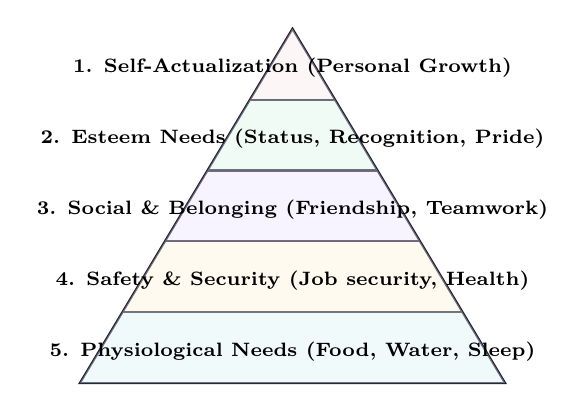
\begin{tikzpicture}[scale=0.9]
  % Triangle Coordinates
  \coordinate (A) at (0,0);
  \coordinate (B) at (6,0);
  \coordinate (C) at (3,5);
  
  \draw[thick, color=mydark] (A) -- (B) -- (C) -- cycle;
  
  % Level 5 (Physiological)
  \draw[thick, color=mydark] (0.6,1) -- (5.4,1);
  \fill[hdrteal, opacity=0.4] (0,0) -- (6,0) -- (5.4,1) -- (0.6,1) -- cycle;
  \node[font=\scriptsize\bfseries] at (3,0.45) {5. Physiological Needs (Food, Water, Sleep)};
  
  % Level 4 (Safety)
  \draw[thick, color=mydark] (1.2,2) -- (4.8,2);
  \fill[hdramber, opacity=0.4] (0.6,1) -- (5.4,1) -- (4.8,2) -- (1.2,2) -- cycle;
  \node[font=\scriptsize\bfseries] at (3,1.45) {4. Safety \& Security (Job security, Health)};
  
  % Level 3 (Social)
  \draw[thick, color=mydark] (1.8,3) -- (4.2,3);
  \fill[hdrpurple, opacity=0.4] (1.2,2) -- (4.8,2) -- (4.2,3) -- (1.8,3) -- cycle;
  \node[font=\scriptsize\bfseries] at (3,2.45) {3. Social \& Belonging (Friendship, Teamwork)};
  
  % Level 2 (Esteem)
  \draw[thick, color=mydark] (2.4,4) -- (3.6,4);
  \fill[hdrgreen, opacity=0.4] (1.8,3) -- (4.2,3) -- (3.6,4) -- (2.4,4) -- cycle;
  \node[font=\scriptsize\bfseries] at (3,3.45) {2. Esteem Needs (Status, Recognition, Pride)};
  
  % Level 1 (Self-Actualization)
  \fill[hdrred, opacity=0.4] (2.4,4) -- (3.6,4) -- (3,5) -- cycle;
  \node[font=\scriptsize\bfseries] at (3,4.45) {1. Self-Actualization (Personal Growth)};
\end{tikzpicture}
\end{tcolorbox}

\subsection{Herzberg's Two-Factor (Dual-Factor) Theory}
Frederick Herzberg proposed that job satisfaction and job dissatisfaction are governed by two distinct sets of factors:
\begin{itemize}[leftmargin=*, itemsep=3.5pt]
  \item \textbf{Hygiene Factors (Dissatisfiers):} Extrinsic job factors (e.g., salary, working conditions, company policy, supervision, relationship with peers).
    *Effect:* If these are missing or poor, they cause extreme dissatisfaction. However, improving them beyond a basic level does not motivate employees or create long-term satisfaction.
  \item \textbf{Motivators (Satisfiers):} Intrinsic job factors (e.g., achievement, recognition, responsibility, growth, the work itself).
    *Effect:* If present, they drive high motivation and job satisfaction. If absent, they do not cause active dissatisfaction, but result in a neutral state.
\end{itemize}

\subsection{McGregor's Theory X and Theory Y}
Douglas McGregor proposed two contrasting sets of assumptions about human nature and worker motivation:
\begin{itemize}[leftmargin=*, itemsep=3.5pt]
  \item \textbf{Theory X (Traditional View):} Assumes employees are inherently lazy, dislike work, avoid responsibility, prefer to be directed, and are motivated primarily by money and security.
    \textit{Management Style:} Autocratic, close supervision, coercive control, and punishment threat.
  \item \textbf{Theory Y (Modern View):} Assumes employees view work as natural as play or rest, are self-directed, seek responsibility, and possess creative potential.
    \textit{Management Style:} Democratic, participative, delegating authority, and self-control.
\end{itemize}

% ===============================================================================
\section{Project Reports: PPR and DPR}
% ===============================================================================

To obtain registration, environmental clearances, and bank funding, an entrepreneur must draft formal feasibility reports.

\subsection{PPR vs. DPR Comparison}
\par\noindent
{\renewcommand{\arraystretch}{1.5}%
\begin{tabularx}{\linewidth}{|B{3.0cm}|Y|Y|}\hline
\multicolumn{1}{|>{\centering\arraybackslash}m{3.0cm}|}{\textbf{Parameter}} &
\multicolumn{1}{>{\centering\arraybackslash}Y|}{\textbf{Preliminary Project Report (PPR)}} &
\multicolumn{1}{>{\centering\arraybackslash}Y|}{\textbf{Detailed Project Report (DPR)}} \\
\hline
\textbf{Objective} & To assess initial feasibility and get provisional registrations. & Final detailed plan used to secure bank loans and equity funds. \\
\hline
\textbf{Scope} & High-level summary of the business idea, raw materials, and cost. & Comprehensive, exhaustive analysis of all technical and financial parameters. \\
\hline
\textbf{Cost \& Time} & Low cost; drafted quickly using secondary data. & Expensive; requires field surveys, expert consultations, and quotes. \\
\hline
\textbf{Financials} & Rough cost estimates and sales targets. & Project balance sheet, cash flow forecasts, IRR, BEP, and payback period. \\
\hline
\end{tabularx}
}

\subsection{Key Contents of a Detailed Project Report (DPR)}
A bankable DPR must contain the following core sections:
\begin{enumerate}[label=\textbf{\arabic*.}, leftmargin=*, itemsep=3pt]
  \item \textbf{General Information:} Promoter profiles, experience, and executive summary.
  \item \textbf{Technical Feasibility:} Raw material specifications, manufacturing technology, plant layout, machinery capacity, power/water requirements, and waste disposal.
  \item \textbf{Market Feasibility:} Competitor analysis, pricing strategy, distribution channels, and sales forecasts.
  \item \textbf{Financial Feasibility:} Total project cost (land, machinery, working capital), financing structure (debt-equity ratio), cash flow statement, projected balance sheets, Net Present Value (NPV), Internal Rate of Return (IRR), and Break-Even Point.
  \item \textbf{Environmental Impact Assessment (EIA):} Waste management planning and pollution control clearances.
\end{enumerate}

\newpage

% ===============================================================================
% MANDATORY QUICK REVISION PAGE
% ===============================================================================
\begin{center}
  {\large\bfseries\color{myred} Quick Revision --- Module 4}\\[3pt]
  {\small\color{mydark} Decision, Motivation \& Project Reports $|$ OE-EC704C}
\end{center}
\noindent{\color{myred}\rule{\linewidth}{1.2pt}}
\vspace{4pt}

\begin{tcolorbox}[formulabox, title={\textbf{Key Concepts \& Equations}}]
\renewcommand{\arraystretch}{1.3}
\begin{tabularx}{\linewidth}{B{4.0cm} X}
Moving Average & $F_{t+1} = \frac{A_t + A_{t-1} + \dots + A_{t-n+1}}{n}$. \\
Exponential Smoothing & $F_{t+1} = \alpha A_t + (1 - \alpha) F_t$. \\
Maslow's Level 1 & Self-Actualization (top level, personal growth). \\
Maslow's Level 5 & Physiological Needs (base level, survival). \\
Hygiene Factors & Extrinsic job variables (dissatisfaction preventers). \\
Motivators & Intrinsic job variables (active satisfaction drivers). \\
Theory X vs. Theory Y & Lazy \& Coerced vs. Self-motivated \& Empowered. \\
\end{tabularx}
\end{tcolorbox}

\begin{tcolorbox}[defbox, title={\textbf{One-Line Definitions}}]
\begin{itemize}[leftmargin=*, itemsep=2.5pt, topsep=0pt]
  \item \textbf{Non-Programmed Decisions:} Decisions addressing novel, unstructured, complex, and high-risk problems.
  \item \textbf{Delphi Method:} Qualitative forecasting using anonymous iterative surveys of an expert panel to reach consensus.
  \item \textbf{Personnel Management:} Attracting, selecting, training, and retaining employees to meet organizational goals.
  \item \textbf{Self-Actualization:} Realizing one's full potential and self-fulfillment (top of Maslow's pyramid).
  \item \textbf{Hygiene Factors:} Extrinsic conditions (like salary and policy) that prevent dissatisfaction but do not motivate.
  \item \textbf{Theory Y:} Management view assuming workers seek responsibility and are self-directed.
  \item \textbf{Detailed Project Report (DPR):} Comprehensive technical and financial plan submitted for bank loan approvals.
\end{itemize}
\end{tcolorbox}

\begin{tcolorbox}[exambox, title={\textbf{Frequently Asked / Viva Questions}}]
\begin{enumerate}[topsep=0pt, label=\textbf{Q\arabic*.}, itemsep=5pt]
  \item \Q{Differentiate between programmed and non-programmed decisions.}
    Programmed decisions are routine, structured, and resolved using established rules (e.g., ordering stationery). Non-programmed decisions are unique, unstructured, and require custom analysis and top-management judgment (e.g., acquiring a competitor).
  \item \Q{State the formula for Exponential Smoothing forecasting and define the terms.}
    $F_{t+1} = F_t + \alpha (A_t - F_t)$, where $F_{t+1}$ is the new forecast, $F_t$ is the current forecast, $A_t$ is the actual demand, and $\alpha$ is the smoothing constant ($0 \le \alpha \le 1$).
  \item \Q{Explain the Delphi method of forecasting.}
    It is a qualitative technique where facilitators send questionnaires to a panel of experts. The experts' anonymous answers are summarized and shared back in multiple rounds, allowing experts to refine opinions until consensus is reached.
  \item \Q{List the five levels of Maslow's Hierarchy of Needs from lowest to highest.}
    Physiological Needs $\rightarrow$ Safety and Security Needs $\rightarrow$ Social and Belongingness Needs $\rightarrow$ Esteem Needs $\rightarrow$ Self-Actualization.
  \item \Q{According to Herzberg, does raising wages motivate employees?}
    No. Wages/Salary are extrinsic \textbf{Hygiene Factors}. Raising them prevents dissatisfaction but does not create long-term motivation. True motivation comes from intrinsic factors like responsibility and recognition.
  \item \Q{What are the assumptions of Douglas McGregor's Theory X?}
    Theory X assumes that the average human dislikes work, avoids responsibility, lacks ambition, prefers to be directed, and must be coerced or threatened with punishment to achieve corporate objectives.
  \item \Q{What is the difference between a PPR and a DPR?}
    A PPR is a brief, low-cost overview used for initial clearance and provisional registration. A DPR is a detailed, comprehensive feasibility report (technical, market, financial) used to secure institutional finance.
  \item \Q{What sections must be included in a Detailed Project Report (DPR)?}
    Promoter profiles, technical feasibility (technology, plant layout), market feasibility (demand, competition), financial feasibility (cost, cash flows, NPV/IRR/BEP), and environmental impact clearances.
  \item \Q{Define the core steps in the selection process of workers.}
    Application screening $\rightarrow$ Selection test $\rightarrow$ Employment interview $\rightarrow$ Reference check $\rightarrow$ Physical medical exam $\rightarrow$ Job offer.
  \item \Q{Explain the concept of Self-Actualization.}
    It is the highest level of human need in Maslow's hierarchy, referring to the desire for self-fulfillment, realizing one's potential, and continuous personal development.
  \end{enumerate}
\end{tcolorbox}


\end{document}
